\section{Local application handler}

\begin{figure}
	\centering
	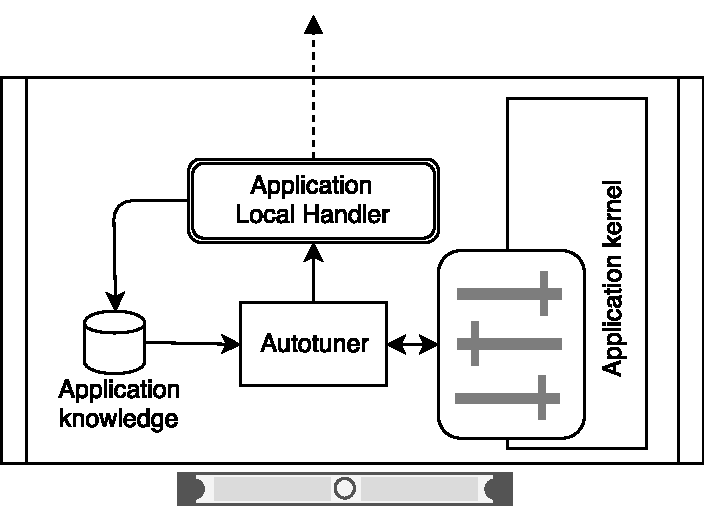
\includegraphics[scale=0.5]{autotuning}
	\caption{The architecture of the local application handler.}
	\label{fig:autotuner}
\end{figure}

The local application handler has three main goals: 1) it provides to the remote application handler information about the actual application, 2) it manages the mARGOt application knowledge to perform a DSE, and 3) provides to mARGOt the final application knowledge.

\prettyref{fig:autotuner} shows the architecture of the local application handler.
While the mARGOt autotuner is synchronous with respect to the execution flow of the target application, the local application handler is a separate thread that communicates with the remote application handler.
In particular, after the initialization, it notifies the existence of a new instance of the application to the server and then it waits for messages.

If the server has no information of this application, the local handler send to the remote handler all the required information.
If the server ask to this client to explore a configuration, the local handler manage the application knowledge to force mARGOt on selecting the given configuration.
If the server send the application knowledge, the local handler replace the old one with the new one.
The only synchronous operation, with respect to the application, happens after each elaboration when mARGOt sends to the remote handler the observed performance of the application.


From the integration point of view, if we are using mARGOt the high-level interface, no additional code is exposed to the end-user.
However, all the required information must be defined in the adaptation configuration file, as described in the mARGOt heel user guide.
